\documentclass{article}
\usepackage{cmap}
\usepackage[utf8]{inputenc}
\usepackage[english,ukrainian]{babel}
\usepackage{graphicx}
\usepackage{geometry}
\usepackage{listings}
\usepackage{float}
\geometry{
	a4paper,
	left=20mm,
	right=20mm,
	top=20mm,
	bottom=20mm
}
\lstset{
	language=c,
	tabsize=4,
	keepspaces,
	showstringspaces=false,
}
\graphicspath{ {./pictures} }
\setlength{\parindent}{4em}

\newcommand\subject{Алгоритми та структури даних}
\newcommand\lecturer{доцент кафедри ПЗ\\Коротєєва Т.О.}
\newcommand\teacher{асистент кафедри ПЗ\\Франко А.В.}
\newcommand\mygroup{ПЗ-22}
\newcommand\lab{6}
\newcommand\theme{Метод сортування підрахунком }
\newcommand\purpose{Вивчити алгоритм сортування підрахунком. Здійснити програмну реалізацію алгоритму сортування підрахунком. Дослідити швидкодію алгоритму сортування підрахунком.}

\begin{document}
	\begin{normalsize}
		\begin{titlepage}
			\thispagestyle{empty}
			\begin{center}
				\textbf{МІНІСТЕРСТВО ОСВІТИ І НАУКИ УКРАЇНИ\\
					НАЦІОНАЛЬНИЙ УНІВЕРСИТЕТ "ЛЬВІВСЬКА ПОЛІТЕХНІКА"}
			\end{center}
			\begin{flushright}
				Інститут \textbf{КНІТ}\\
				Кафедра \textbf{ПЗ}
			\end{flushright}
			\vspace{200pt}
			\begin{center}
				\textbf{ЗВІТ}\\
				\vspace{10pt}
				До лабораторної роботи № \lab\\
				\textbf{На тему}: “\textit{\theme}”\\
				\textbf{З дисципліни}: “\subject”
			\end{center}
			\vspace{112pt}
			\begin{flushright}
				
				\textbf{Лектор}:\\
				\lecturer\\
				\vspace{28pt}
				\textbf{Виконав}:\\
				
				студент групи \mygroup\\
				Коваленко Д.М.\\
				\vspace{28pt}
				\textbf{Прийняв}:\\
				
				\teacher\\
				
				\vspace{28pt}
				«\rule{1cm}{0.15mm}» \rule{1.5cm}{0.15mm} 2022 р.\\
				$\sum$ = \rule{1cm}{0.15mm}……………\\
				
			\end{flushright}
			\vspace{\fill}
			\begin{center}
				\textbf{Львів — 2022}
			\end{center}
		\end{titlepage}
		
		\begin{description}
			\item[Тема.] \theme.
			\item[Мета.] \purpose.
		\end{description}
		
		\section*{Лабораторне завдання}
		Створити віконний проект та написати програму, яка реалізує алгоритм сортування Шелла.
		\begin{center}
			5. Задано одномірний масив дійсних чисел. Виключити з нього моду (елемент, який повторюється найчастіше). Отриманий масив посортувати в порядку зростання..
		\end{center}
		
		\section*{Теоретичні відомості}
	Сортування підрахунком (англійською «Counting Sort») — алгоритм впорядкування, що застосовується при малій кількості різних елементів (ключів) у масиві даних. Час його роботи лінійно залежить як від загальної кількості елементів у масиві так і від кількості різних елементів.
	
	Ідея алгоритму полягає в наступному: спочатку підрахувати скільки разів кожен елемент (ключ) зустрічається в вихідному масиві. Спираючись на ці дані можна одразу вирахувати на якому місці має стояти кожен елемент, а потім за один прохід поставити всі елементи на свої місця.
	
	В алгоритмі присутні тільки прості цикли довжини N (довжина масиву), та один цикл довжини K (величина діапазону). Отже, обчислювальна складність роботи алгоритму становить O(N + K).
	
	В алгоритмі використовується додатковий масив. Тому алгоритм потребує E(K) додаткової пам’яті.
	
	В такій реалізації алгоритм є стабільним. Саме ця його властивість дозволяє використовувати його як частину інших алгоритмів сортування (наприклад, сортування за розрядами).
	
	Використання даного алгоритму є доцільним тільки у випадку малих K.
		
		\subsection*{Покроковий опис роботи алгоритму сортування злиттям}
		\textbf{Алгоритм S - сортування злиттям}
		\begin{enumerate}  
			\item [\textbf{S1}] Цикл по елементах масиву R, i=1…n. Повторювати S2.
			\item [\textbf{S2}] Збільшити значення комірки масиву numbercount з індексом $R_i$.
			\item [\textbf{S3}] Цикл по елементах масиву numbercount. Повторювати S5.
			\item [\textbf{S4}] Додати значення i до масиву answernumbercount i разів.
			\item [\textbf{S5}] Кінець.
		\end{enumerate}
		
		\newpage
		
		\section*{Хід роботи}
		\subsection*{Файл sort.rs}
		\begin{lstlisting}
use crate::data::Data;
use crate::log;

fn get_max(arr: &mut Vec<Data>) -> usize {
	let mut temp: usize = arr[0].v;
	for i in 1..arr.len() {
		if temp < arr[i].v {
			temp = arr[i].v;
		}
	}
	return temp;
}

fn get_min(arr: &mut Vec<Data>) -> usize {
	let mut temp: usize = arr[0].v;
	for i in 1..arr.len() {
		if temp > arr[i].v {
			temp = arr[i].v;
		}
	}
	return temp;
}

pub fn sort(arr: &mut Vec<Data>, res: &mut Vec<Vec<Data>>) {
	let min: usize = get_min(arr);
	let max: usize  = get_max(arr);
	let mut z: usize = 0;
	
	let mut count = vec![0; max - min +1];
	
	for i in 0..arr.len() {
		count[arr[i].v - min] = count[arr[i].v - min] + 1;
	}
	
	for i in min..max+1 {
		while count[i - min] > 0 {
			arr[z].v = i;
			z += 1;
			count[i - min] = count[i - min] - 1;
			res.push(arr.clone());
		}
	}
}


\end{lstlisting}
		
		\section*{Результат роботи}
		\begin{figure}[H]
			\centering
			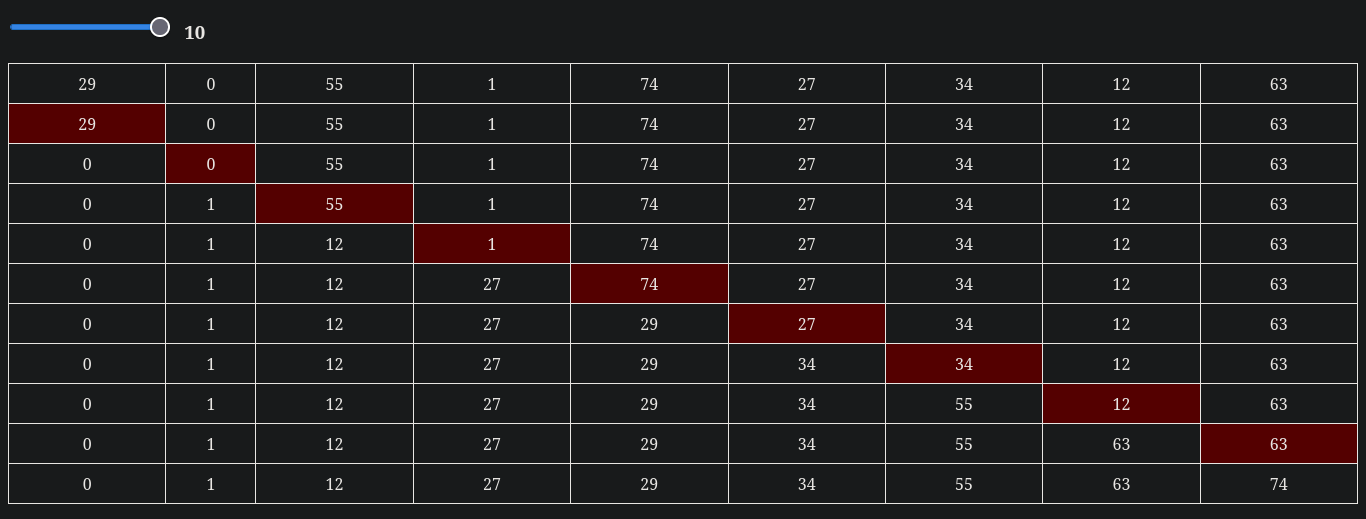
\includegraphics[scale=0.36]{1}
			\caption{Виконання програми}
		\end{figure}
		
		\section*{Висновок}
		Під час виконання лабораторної роботи я вивчив алгоритм сортування підрахунком. Здійснив програмну реалізацію алгоритму сортування підрахунком. Дослідив швидкодію алгоритму сортування підрахунком..
		
	\end{normalsize}
\end{document}
